\documentclass[12pt,fleqn]{article}
\usepackage{vkCourseML}
\hypersetup{unicode=true}
%\usepackage[a4paper]{geometry}
\usepackage[hyphenbreaks]{breakurl}

\interfootnotelinepenalty=10000

\begin{document}
\title{Лекция 3\\Линейная регрессия}
\author{Е.\,А.\,Соколов\\ФКН ВШЭ}
\maketitle

\section{Переобучение}

Мы выработали достаточно общий метод обучения линейных регрессионных моделей,
основанный на градиентных методах оптимизации.
При этом модель может оказаться~\emph{переобученной}~--- её качество
на новых данных может быть существенно хуже качества на обучающей выборке.
Действительно, при обучении мы требуем от модели лишь хорошего качества на обучающей выборке,
и совершенно не очевидно, почему она должна при этом хорошо~\emph{обобщать} эти результаты
на новые объекты.

\begin{figure}[t]
    \centering
    \includegraphics[width=\textwidth]{underfitting_overfitting.eps}
    \caption{Регрессионные кривые для признаковых наборов различной сложности.}
    \label{fig:overfitting}
\end{figure}

В следующем разделе мы обсудим подходы к оцениванию обобщающей способности,
а пока разберём явление переобучения на простом примере.
Рассмотрим некоторую одномерную выборку, значения единственного признака~$x$
в которой генерируются равномерно на отрезке~$[0, 1]$,
а значения целевой переменной выбираются по формуле~$y = \cos(1.5 \pi x) + \mathcal{N}(0, 0.01)$,
где~$\mathcal{N}(\mu, \sigma^2)$~--- нормальное распределение со средним~$\mu$ и дисперсией~$\sigma^2$.
Попробуем восстановить зависимость с помощью линейных моделей над тремя наборами признаков:
$\{x\}$, $\{x, x^2, x^3, x^4\}$ и $\{x, x^2, \dots, x^{15}\}$.
Соответствующие результаты представлены на рис.~\ref{fig:overfitting}.

Видно, что при использовании признаков высоких степеней модель получает возможность
слишком хорошо подстроиться под выборку, из-за чего становится непригодной для дальнейшего использования.
Эту проблему можно решать многими способами~--- например, использовать более узкий класс моделей
или штрафовать за излишнюю сложность полученной модели.
Так, можно заметить, что у переобученной модели, полученной на третьем наборе признаков,
получаются очень большие коэффициенты при признаках.
Как правило, именно норма вектора коэффициентов используется как величина,
которая штрафуется для контроля сложности модели.
Такой подход называется~\emph{регуляризацией}, речь о нём пойдёт ниже.

\section{Оценивание качества моделей}

В примере, о котором только что шла речь, мы не можем обнаружить переобученность модели
по обучающей выборке~\footnote{Конечно, это можно было бы заметить по большим весам в модели,
но связь между нормой весов и обобщающей способностью алгоритма неочевидна.}.
С другой стороны, если бы у нас были дополнительные объекты с известными ответами,
то по ним заметить низкое качество модели было бы довольно легко.

На данной идее основан подход с~\emph{отложенной выборкой}.
Имеющиеся размеченные данные~(т.е. данные с известными ответами)
разделяются на две части: обучающую и контрольную.
На обучающей выборке, как это следует из названия, модель обучается,
а на контрольной выборке проверяется её качество.
Если значение функционала на контрольной выборке оказалось удовлетворительным,
то можно считать, что модель смогла извлечь закономерности при обучении.

Использование отложенной выборки приводит к одной существенной проблеме:
результат существенно зависит от конкретного разбиения данных на обучение и контроль.
Мы не знаем, какое качество получилось бы, если бы объекты из данного
контроля оказались в обучении.
Решить эту проблему можно с помощью~\emph{кросс-валидации}.
Размеченные данные разбиваются на~$k$ блоков~$X_1, \dots, X_k$ примерно одинакового размера.
Затем обучается~$k$ моделей~$a_1(x), \dots, a_k(x)$, причём~$i$-я модель обучается на объектах из всех блоков,
кроме блока~$i$.
После этого качество каждой модели оценивается по тому блоку, который не участвовал в её обучении,
и результаты усредняются:
\[
    \text{CV}
    =
    \frac{1}{k}
    \sum_{i = 1}^{k}
        Q\left( a_i(x), X_i \right).
\]

\section{Регуляризация}

Выше мы упоминали, что если матрица~$X^T X$ не является обратимой,
то с оптимизацией среднеквадратичной ошибки могут возникнуть некоторые трудности.
Действительно, в ряде случаев (признаков больше чем объектов, коррелирующие признаки)
оптимизационная задача~$Q(w) \to \min$ может иметь бесконечное число решений,
большинство которых являются переобученными и плохо работают на тестовых данных.
Покажем это.

Пусть в выборке есть линейно зависимые признаки.
Это по определению означает, что существует такой вектор~$v$,
что для любого объекта~$x$ выполнено~$\langle v, x \rangle = 0$.
Допустим, мы нашли оптимальный вектор весов~$w$ для линейного классификатора.
Но тогда классификаторы с векторами~$w + \alpha v$ будут давать~\emph{точно такие же}
ответы на всех объектах, поскольку
\[
    \langle w + \alpha v, x \rangle
    =
    \langle w, x \rangle
    +
    \alpha
    \underbrace{
        \langle v, x \rangle
    }_{=0}
    =
    \langle w, x \rangle.
\]
Это значит, что метод оптимизации может найти решение
со сколько угодно большими весами.
Такие решения не очень хороши, поскольку классификатор
будет чувствителен к крайне маленьким изменениям
в признаках объекта, а значит, переобучен.

Мы уже знаем, что переобучение нередко приводит к большим значениям коэффициентов.
Чтобы решить проблему, добавим к функционалу~\emph{регуляризатор},
который штрафует за слишком большую норму вектора весов:
\[
    Q_\alpha(w) = Q(w) + \alpha R(w).
\]

Наиболее распространенными являются~$L_2$ и~$L_1$-регуляризаторы:
\begin{align*}
    &R(w) = \|w\|_2 = \sum_{i = 1}^d w_i^2, \\
    &R(w) = \|w\|_1 = \sum_{i = 1}^d |w_i|.
\end{align*}

Коэффициент~$\alpha$ называется параметром регуляризации и контролирует баланс между
подгонкой под обучающую выборку и штрафом за излишнюю сложность.
Разумеется, значение данного параметра следует подбирать под каждую задачу.

Отметим, что свободный коэффициент~$w_0$ нет смысла регуляризовывать~---
если мы будем штрафовать за его величину, то получится, что
мы учитываем некие априорные представления о близости целевой переменной к нулю
и отсутствии необходимости в учёте её смещения.
Такое предположение является достаточно странным.
Особенно об этом следует помнить, если в выборке есть константный признак
и коэффициент~$w_0$ обучается наряду с остальными весами;
в этом случае следует исключить слагаемое, соответствующее константному признаку, из регуляризатора.

Квадратичный~(или~$L_2$) регуляризатор достаточно прост в использовании
в отличие от~$L_1$-регуляризатора, у которого нет производной в нуле.
При этом~$L_1$-регуляризатор имеет интересную особенность:
его использование приводит к занулению части весов.
Позже мы подробно обсудим это явление.

Обратим внимание на вид решения при использовании~$L_2$-регуляризации вместе со среднеквадратичной ошибкой.
В этом случае формулу для оптимального вектора весов можно записать в явном виде:
\[
    w
    =
    (X^T X + \alpha I)^{-1} X^T y.
\]
Благодаря добавлению диагональной матрицы к~$X^T X$ данная матрица
оказывается положительно определённой, и поэтому её можно обратить.
Таким образом, при использовании~$L_2$ регуляризации решение всегда будет единственным.

\section{Гиперпараметры}

В машинном обучении принято разделять подлежащие настройке величины
на~\emph{параметры} и~\emph{гиперпараметры}.
Параметрами называют величины, которые настраиваются по обучающей выборке~--- например,
веса в линейной регрессии.
К гиперпараметрам относят величины, которые контролируют сам процесс обучения и
не могут быть подобраны по обучающей выборке.

Хорошим примером гиперпараметра является коэффициент регуляризации~$\alpha$.
Введение регуляризации мешает модели подгоняться под обучающие данные,
и с точки зрения среднеквадратичной ошибки выгодно всегда брать~$\alpha = 0$.
Разумеется, такой выбор не будет оптимальным с точки зрения качества на новых данных,
и поэтому коэффициент регуляризации~(как и другие гиперпараметры) следует
настраивать по отложенной выборке или с помощью кросс-валидации.

При подборе гиперпараметров по кросс-валидации возникает проблема:
мы используем отложенные данные, чтобы выбрать лучший набор гиперпараметров.
По сути, отложенная выборка тоже становится обучающей, и показатели качества на ней
перестают характеризовать обобщающую способность модели.
В таких случаях выборку, на которой настраиваются гиперпараметры,
называют валидационной, и при этом выделяют третий, тестовый набор данных,
на которых оценивается качество итоговой модели.

\section{Разреженные модели}

В процессе обсуждения регуляризации мы упомянули, что использование~$L_1$-регуляризатора
приводит к обнулению части весов в модели.
Обсудим подробнее, зачем это может понадобиться и почему так происходит.

Модели, в которых некоторые веса равны нулю, называют~\emph{разреженными},
поскольку прогноз в них зависит лишь от части признаков.
Потребность в таких моделях можно возникнуть по многим причинам.
Несколько примеров:
\begin{enumerate}
    \item Может быть заведомо известно, что релевантными являются не все признаки.
        Очевидно, что признаки, которые не имеют отношения к задаче, надо исключать из данных,
        то есть производить~\emph{отбор признаков}.
        Есть много способов решения этой задачи, и~$L_1$-регуляризация~--- один из них.
    \item К модели могут выдвигаться ограничения по скорости построения предсказаний.
        В этом случае модель должна зависеть от небольшого количества наиболее важных признаков,
        и тут тоже оказывается полезной~$L_1$-регуляризация.
    \item В обучающей выборке объектов может быть существенно меньше, чем признаков~(так называемая~<<проблема $N \ll p$>>).
        Поскольку параметров линейной модели при этом тоже больше, чем объектов, задача обучения оказывается
        некорректной~--- решений много, и сложно выбрать из них то, которое обладает
        хорошей обобщающей способностью.
        Решить эту проблему можно путём внедрения в процесс обучения априорного знания о том,
        что целевая переменная зависит от небольшого количества признаков.
        Такая модификация как раз может быть сделана с помощью~$L_1$-регуляризатора.
\end{enumerate}
Теперь, когда мы представляем некоторые области применения разреженных моделей,
попробуем понять, почему~$L_1$ регуляризатор позволяет их обучать.
Этому есть несколько объяснений.

\begin{figure}[t]
    \centering
    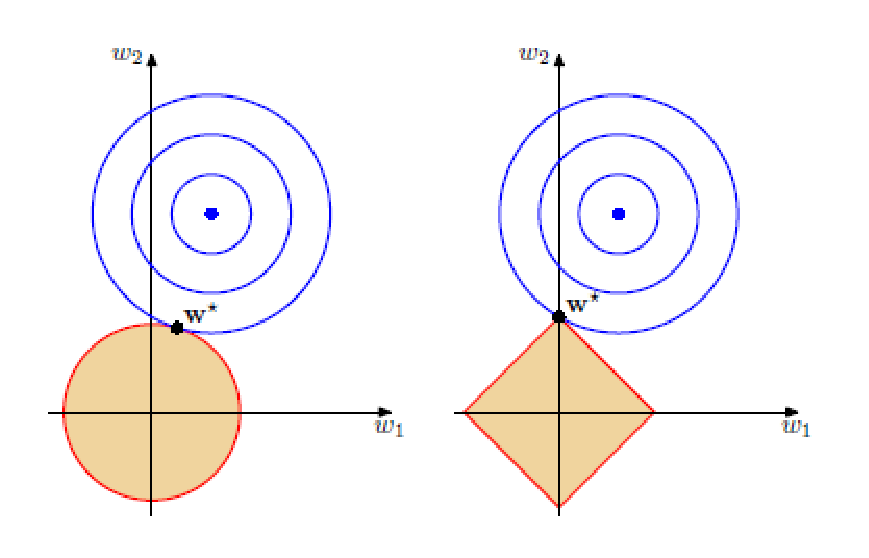
\includegraphics[width=0.5\linewidth]{reg.eps}
    \caption{Линии уровня функционала качества, а также ограничения,
        задаваемые~$L_2$ и~$L_1$-регуляризаторами.}
    \label{pic:regularizers}
\end{figure}

\paragraph{Угловые точки.}
Можно показать, что если функционал~$Q(w)$ является выпуклым,
то задача безусловной минимизации функции~$Q(w) + \alpha \|w\|_1$
эквивалентна задаче условной оптимизации
\[
    \left\{
        \begin{aligned}
            & Q(w) \to \min_{w} \\
            & \|w\|_1 \leq C
        \end{aligned}
    \right.
\]
для некоторого~$C$.
На рис.~\ref{pic:regularizers}
изображены линии уровня функционала~$Q(w)$,
а также множество, определяемое ограничением~$\|w\|_1 \leq C$.
Решение определяется точкой пересечения допустимого множества с линией уровня,
ближайшей к безусловному минимуму.
Из изображения можно предположить, что в большинстве случаев эта точка будет лежать на одной из вершин ромба,
что соответствует решению с одной зануленной компонентой.

\paragraph{Штрафы при малых весах.}
Предположим, что текущий вектор весов состоит из двух элементов~$w = (1, \eps)$,
где~$\eps$ близко к нулю,
и мы хотим немного изменить данный вектор по одной из координат.
Найдём изменение~$L_2$- и~$L_1$-норм вектора при уменьшении первой компоненты на некоторое
положительное число~$\delta < \eps$:
\begin{align*}
    &\|w - (\delta, 0)\|_2^2
    =
    1 - 2 \delta + \delta^2 + \eps^2\\
    &\|w - (\delta, 0)\|_1
    =
    1 - \delta + \eps
\end{align*}
Вычислим то же самое для изменения второй компоненты:
\begin{align*}
    &\|w - (0, \delta)\|_2^2
    =
    1 - 2 \eps \delta + \delta^2 + \eps^2\\
    &\|w - (0, \delta)\|_1
    =
    1 - \delta + \eps
\end{align*}

Видно, что с точки зрения~$L_2$-нормы выгоднее уменьшать первую компоненту,
а для~$L_1$-нормы оба изменения равноценны.
Таким образом, при выборе~$L_2$-регуляризации гораздо меньше шансов,
что маленькие веса будут окончательно обнулены.

\paragraph{Проксимальный шаг.}
\emph{Проксимальные методы}~--- это класс методов оптимизации, которые
хорошо подходят для функционалов с негладкими слагаемыми.
Не будем сейчас останавливаться на принципах их работы, а приведём лишь
формулу для шага проксимального метода в применении к линейной регрессии
с квадратичным функционалом ошибки и~$L_1$-регуляризатором:
\[
    w^{(k)}
    =
    S_{\eta \alpha} \left(
        w^{(k - 1)}
        -
        \eta
        \nabla_w F(w^{(k - 1)})
    \right),
\]
где~$F(w) = \|Xw - y\|^2$~--- функционал ошибки без регуляризатора,
$\eta$~--- длина шага,
$\alpha$~--- коэффициент регуляризации,
а функция~$S_{\eta \alpha}(w)$ применяется к вектору весов покомпонентно,
и для одного элемента выглядит как
\[
    S_{\eta \alpha} (w_i)
    =
    \begin{cases}
        w_i - \eta \alpha, \quad &w_i > \eta \alpha\\
        0, \qquad &|w_i| < \eta \alpha\\
        w_i + \eta \alpha, \quad &w_i < -\eta \alpha
    \end{cases}
\]
Из формулы видно, что если на данном шаге значение некоторого веса не очень большое,
то на следующем шаге этот вес будет обнулён, причём чем больше коэффициент регуляризации,
тем больше весов будут обнуляться.

\section{Квантильная регрессия}
В некоторых задачах цены занижения и завышения прогнозов могут отличаться друг от друга.
Например, при прогнозировании спроса на товары интернет-магазина гораздо опаснее заниженные
предсказания, поскольку они могут привести к потере клиентов.
Завышенные же прогнозы приводят лишь к издержкам на хранение товара на складе.
Функционал в этом случае можно записать как
\[
    Q(a, X^\ell)
    =
    \sum_{i = 1}^{\ell}
        \rho_\tau(y_i - a(x_i)),
\]
где
\[
    \rho_\tau(z)
    =
    (\tau - 1) [z < 0] z
    +
    \tau [z \geq 0] z,
\]
а параметр~$\tau$ лежит на отрезке~$[0, 1]$ и определяет
соотношение важности занижения и завышения прогноза.
Чем больше здесь~$\tau$, тем выше штраф за занижение прогноза.

На семинарах будет показано, что если алгоритм должен выдавать константу,
то при таком функционале оптимально будет возвращать~$\tau$-квантиль по всем ответам.
Сейчас же обсудим вероятностный смысл данного функционала.
Будем считать, что в каждой точке~$x \in \XX$ пространства объектов
задано вероятностное распределение~$p(y \cond x)$ на возможных ответах для данного объекта.
Такое распределение может возникать, например, в задаче предсказания кликов по рекламным баннерам:
один и тот же пользователь может много раз заходить на один и тот же сайт и видеть данный баннер;
при этом некоторые посещения закончатся кликом, а некоторые~--- нет.

Известно, что при оптимизации квадратичного функционала алгоритм~$a(x)$
будет приближать условное матожидание ответа в каждой точке пространства
объектов:~$a(x) \approx \EE [y \cond x]$;
если же оптимизировать среднее абсолютное отклонение, то итоговый алгоритм
будет приближать медиану распределения:~$a(x) \approx \text{median} [p(y \cond x)]$.
Рассмотрим теперь некоторый объект~$x$ и условное распределение~$p(y \cond x)$.
Найдем  число~$q$, которое будет оптимальным с точки зрения нашего функционала:
\[
    Q = \int_\YY \rho_\tau(y - q) p(y \cond x) dy.
\]
Продифференцируем его~(при этом необходимо воспользоваться правилами
дифференцирования интегралов, зависящих от параметра):
\[
    \frac{\partial Q}{\partial q}
    =
    (1 - \tau) \int_{-\infty}^{q} p(y \cond x) dy
    -
    \tau \int_{q}^{\infty} p(y \cond x) dy
    =
    0.
\]
Получаем, что
\[
    \frac{\tau}{1 - \tau}
    =
    \frac{
        \int_{-\infty}^{q} p(y \cond x) dy
    }{
        \int_{q}^{\infty} p(y \cond x) dy
    }.
\]
Данное уравнение будет верно, если~$q$ будет равно~$\tau$-квантили распределения~$p(y \cond x)$.
Таким образом, использование функции потерь~$\rho_\tau(z)$ приводит к тому,
что алгоритм~$a(x)$ будет приближать~$\tau$-квантиль распределения ответов в каждой точке
пространства объектов.

\section{Преобразования признаков}

\subsection{Нелинейные признаки}

С помощью линейной регрессии можно восстанавливать нелинейные зависимости,
если провести преобразование признакового пространства:
\[
    x = (x_1, \dots, x_d) \to \phi(x) = (\phi_1(x), \dots, \phi_m(x)).
\]
Например, можно перейти к квадратичным признакам:
\[
    \phi(x)
    =
    (x_1, \dots, x_d, x_1^2, \dots, x_d^2, x_1 x_2, \dots, x_{d-1} x_d).
\]
Линейная модель над новыми признаками уже сможет приближать любые квадратичные закономерности.
Аналогично можно работать и с полиномиальными признаками более высоких порядков.

Возможны и другие преобразования:
\begin{itemize}
    \item $\log x_j$~--- для признаков с тяжёлыми хвостами
    \item $\exp(\|x - \mu\|^2 / \sigma)$~--- для измерения близости до некоторой точки
    \item $\sin(x_j / T)$~--- для задач с периодическими зависимостями
\end{itemize}

\subsection{Масштабирование}

\begin{figure}[t]
    \centering
    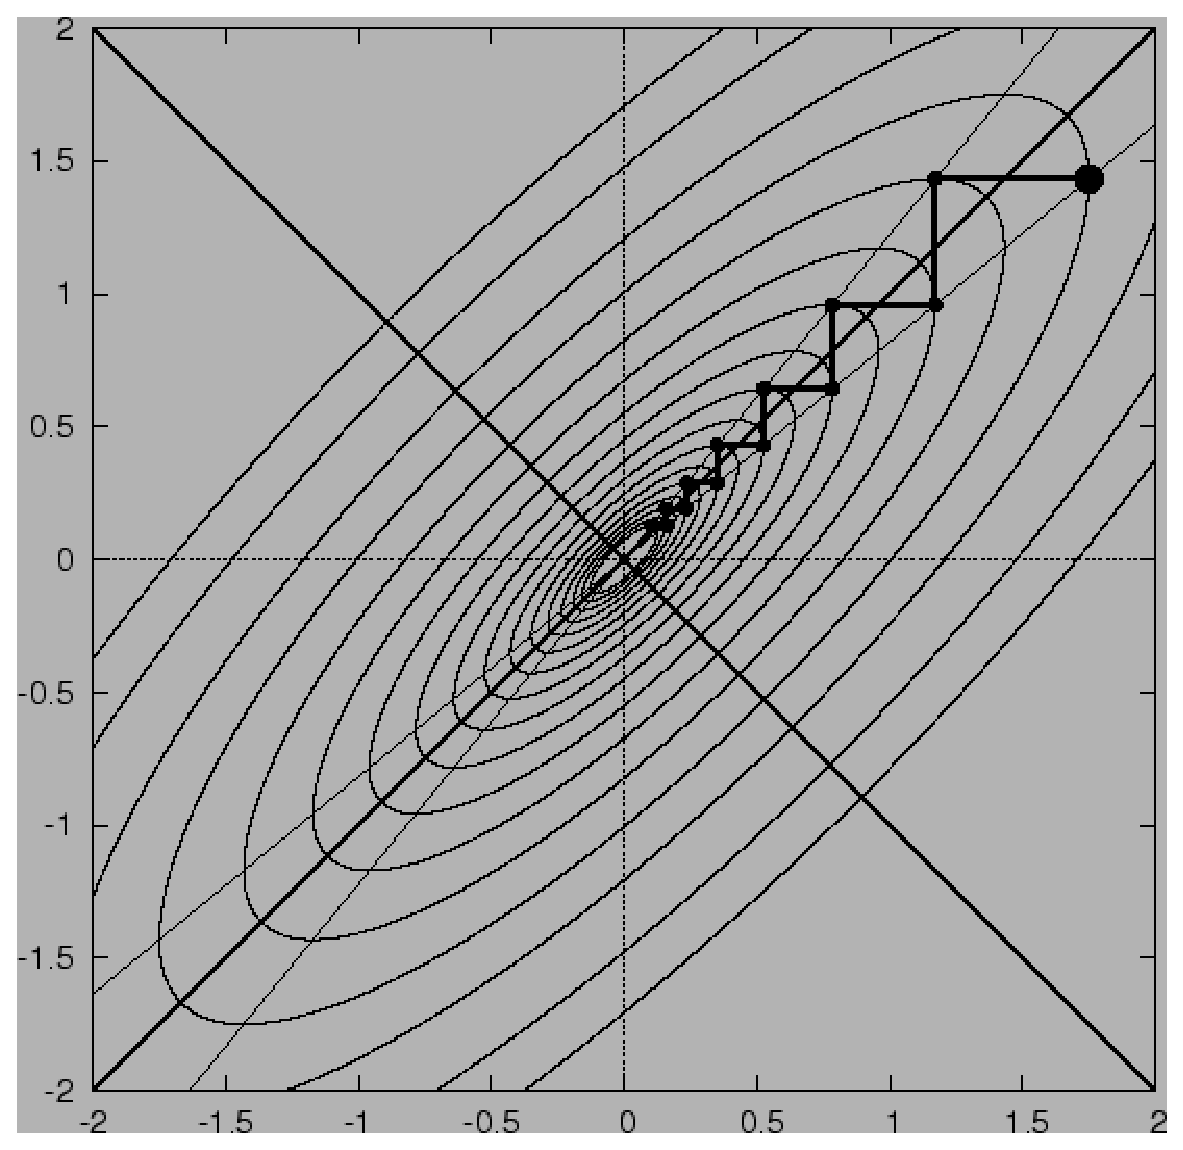
\includegraphics[width=0.4\linewidth]{descent.eps}
    \caption{Траектория градиентного спуска на функционале при признаках разного масштаба.}
    \label{pic:descent}
\end{figure}

При обучении линейных моделей полезно масштабировать признаки, то есть приводить их к единой шкале.
Разберёмся, зачем это нужно.

Рассмотрим функцию~$f_1(x) = \frac{1}{2} x_1^2 + \frac{1}{2} x_2^2$, выберем начальное приближение~$x^{(0)} = (1, 1)$
и запустим из него градиентный спуск с параметром $\eta = 1$.
Окажется, что за один шаг мы сможем сразу попасть в точку минимума.

Теперь~<<растянем>> функцию вдоль одной из осей:~$f_2(x) = 50 x_1^2 + \frac{1}{2} x_2^2$.
При таком же начальном приближении~$x^{(0)}$ антиградиент на первой итерации будет равен~$(-100, -1)$,
и попасть по нему в минимум уже невозможно~--- более того, при неаккуратном выборе длины шага можно
очень далеко уйти от минимума.
Пример траектории градиентного спуска при такой форме функции можно найти на рис.~\ref{pic:descent}.

Аналогичная проблема возникает с функционалом ошибки в линейной регрессии, если один из признаков
существенно отличается по масштабу от остальных.
Чтобы избежать этого, признаки следует масштабировать~--- например, путём стандартизации:
\[
    x_{ij}
    :=
    \frac{x_{ij} - \mu_j}{\sigma_j},
\]
где~$\mu_j = \frac{1}{\ell} \sum_{i = 1}^{\ell} x_{ij}$,
$\sigma_j = \frac{1}{\ell} \sum_{i = 1}^{\ell} (x_{ij} - \mu_j)^2$.
Или, например, можно масштабировать признаки на отрезок~$[0, 1]$:
\[
    x_{ij}
    :=
    \frac{x_{ij} - \min_i x_{ij}}{\max_i x_{ij} - \min_i x_{ij}}.
\]

\end{document}
